\begin{question}
\noindent On a coordinate plane used to design an e-sports tournament bracket display, triangle $A$ has vertices $A_1(-5,1)$, $A_2(-5,3)$, $A_3(-2,1)$.

\begin{center}
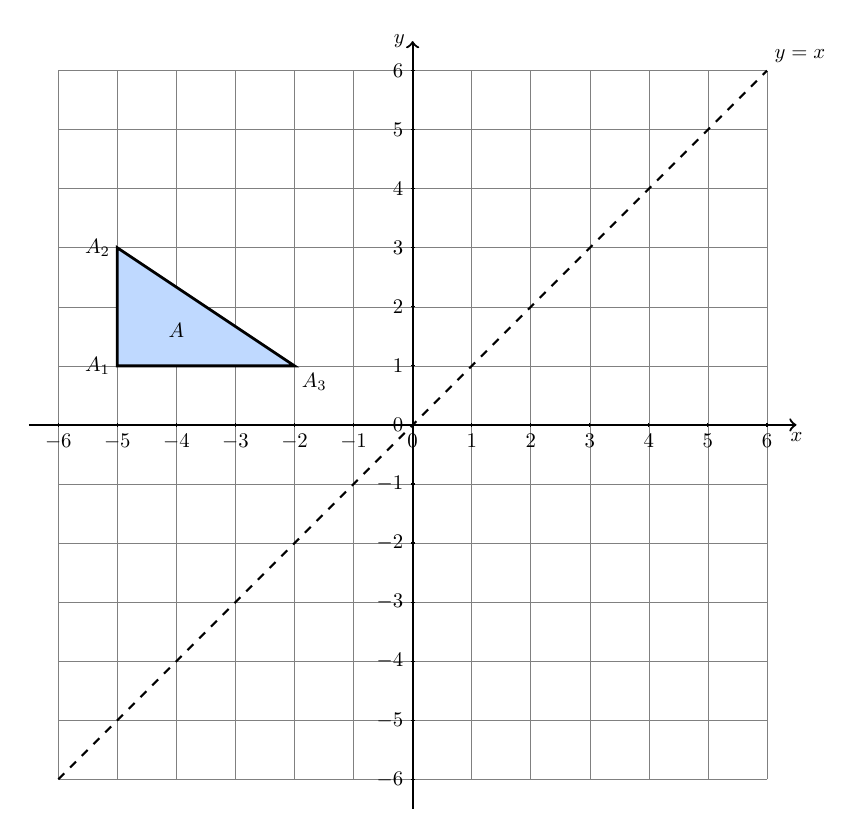
\begin{tikzpicture}[scale=0.75, transform shape]
    \def\axisLimit{6}

    \definecolor{borderColour}{HTML}{000000}
    \definecolor{fillColourA}{HTML}{BFD9FF}

    % Draw grid
    \draw[step=1cm,gray,very thin] (-\axisLimit,-\axisLimit) grid (\axisLimit,\axisLimit);

    % Draw axes
    \draw[thick,->] (-\axisLimit-0.5,0) -- (\axisLimit+0.5,0) node[anchor=north] {$x$};
    \draw[thick,->] (0,-\axisLimit-0.5) -- (0,\axisLimit+0.5) node[anchor=east] {$y$};

    % Label x-axis and y-axis
    \foreach \x in {-\axisLimit,...,\axisLimit}
        \draw (\x cm,1pt) -- (\x cm,-1pt) node[anchor=north] {$\x$};
    \foreach \y in {-\axisLimit,...,\axisLimit}
        \draw (1pt,\y cm) -- (-1pt,\y cm) node[anchor=east] {$\y$};

    % Triangle A: (-5,1), (-5,3), (-2,1)
    \coordinate (A1) at (-5,1);
    \coordinate (A2) at (-5,3);
    \coordinate (A3) at (-2,1);
    \filldraw[fill=fillColourA, draw=borderColour, line width=1pt] (A1) -- (A2) -- (A3) -- cycle;
    \node[left] at (A1) {$A_1$};
    \node[left] at (A2) {$A_2$};
    \node[below right] at (A3) {$A_3$};
    \node at (-4,1.6) {$A$};

    % Draw the line y = x for part (b)
    \draw[thick, dashed] (-6,-6) -- (6,6) node[anchor=south west] {$y=x$};

\end{tikzpicture}
\end{center}

\begin{enumerate}
    \item[(a)] Triangle $A$ is translated by the vector $\begin{pmatrix}4\\-5\end{pmatrix}$ to give triangle $B$.

    Find the coordinates of the vertices of triangle $B$.

    \vspace{4cm}
    \answerplain{2}

    \item[(b)] Triangle $B$ is then reflected in the line $y = x$ to give triangle $C$.

    Find the coordinates of the vertices of triangle $C$.

    \vspace{4cm}
    \answerplain{2}
\end{enumerate}
\end{question}
